\section{How does the decline of HPV is affected if the average number of LSPs increases significantly?}

The data used to build the network model and to perform the calibration have more than $10$ years. Also, the sexual behavior of the people has changed a lot in the last years and therefore, it would be interesting to perform some simulations adapting the model parameters to the new sexual behavior. Here, we propose an increasing in the number of lifetime sexual partners (LSP) of the nodes.

In Table \ref{table:laselegidas} in page \pageref{table:laselegidas} we determined by model calibration that the average LSP of men are $8.63$ with $95\%$ confidence interval $[7.15, 9.86]$. These values were selected during the calibration and correspond to the $30$  realizations appearing in (\ref{laselegidas}). Each realization has associated model parameters, in particular, its average LSP men.

Here, we are going to sum 4 to the $30$ average LSP men, increasing in 4 the number of average LSP. Only girls are vaccinated with a $70\%$ coverage (Spanish current program).

In Figure \ref{fig:compara_k} we can see graphically the obtained results. 

\begin{figure}[!]
	\centering
	\begin{tabular}{cc}
		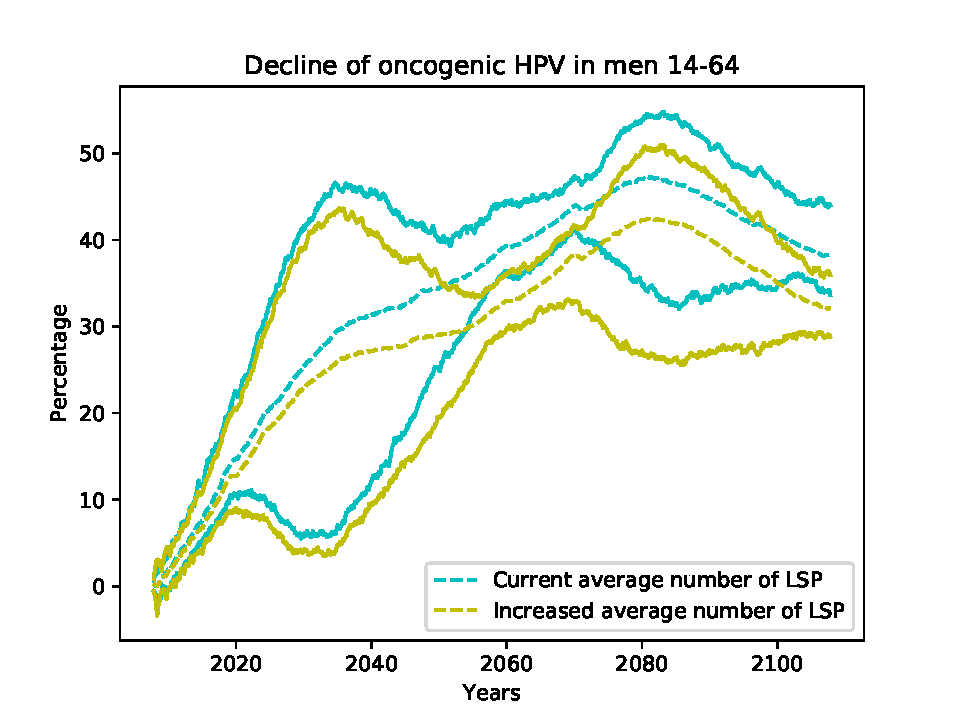
\includegraphics[width=0.5\linewidth]{IMGs/12.-Aumento_LSP/onco_hom.pdf}	& 
		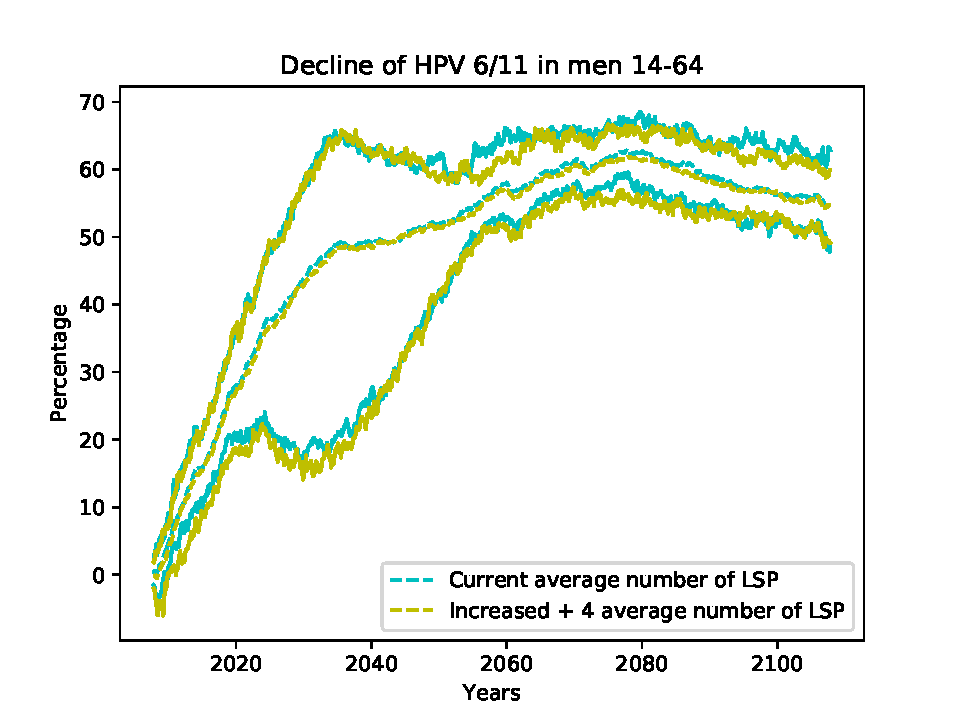
\includegraphics[width=0.5\linewidth]{IMGs/12.-Aumento_LSP/verr_hom.pdf}  \\ 
		Decline oncogenic HPV men	& Decline HPV 6/11 men \\ 
		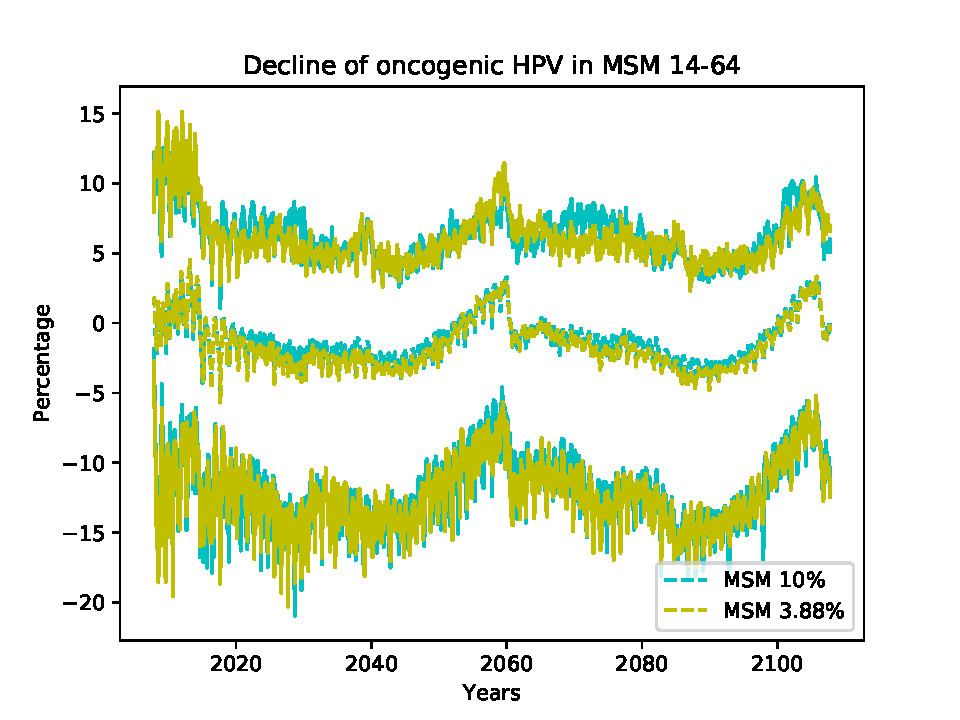
\includegraphics[width=0.5\linewidth]{IMGs/13.-Aumento_MSM/onco_MSM.pdf}	& 
		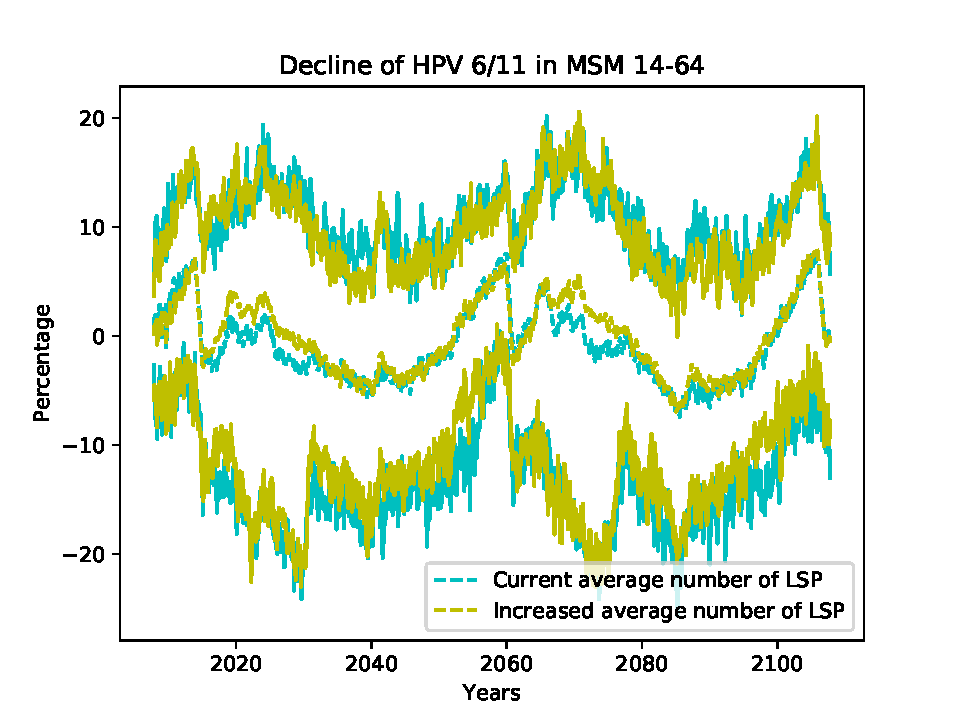
\includegraphics[width=0.5\linewidth]{IMGs/12.-Aumento_LSP/verr_MSM.pdf}  \\ 
		Decline oncogenic HPV MSM	& Decline HPV 6/11 MSM \\ 
		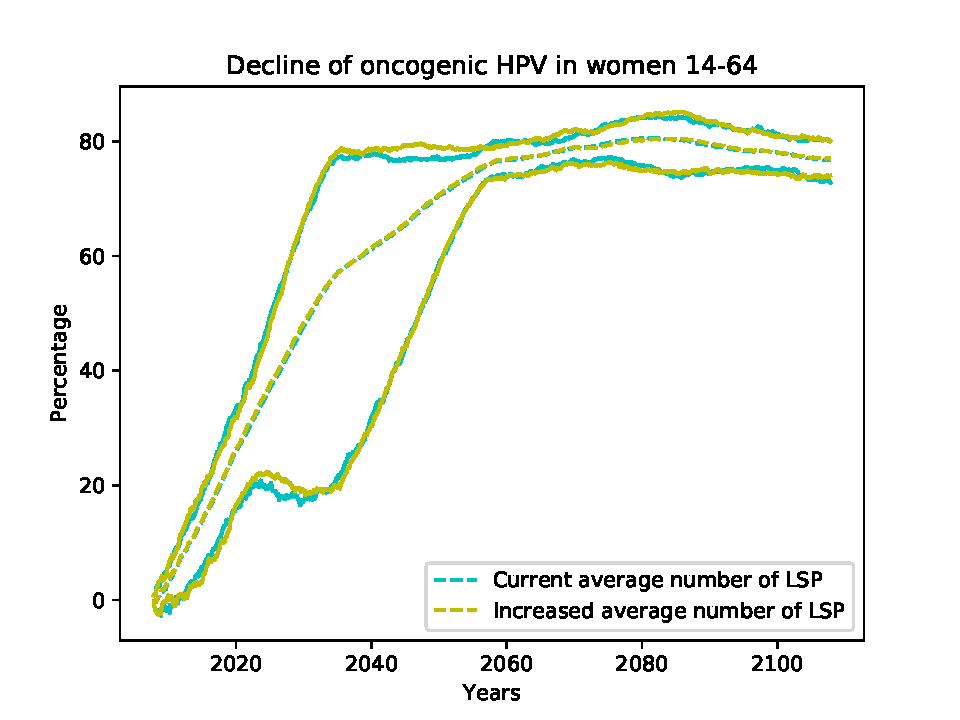
\includegraphics[width=0.5\linewidth]{IMGs/12.-Aumento_LSP/onco_muj.pdf}	& 
		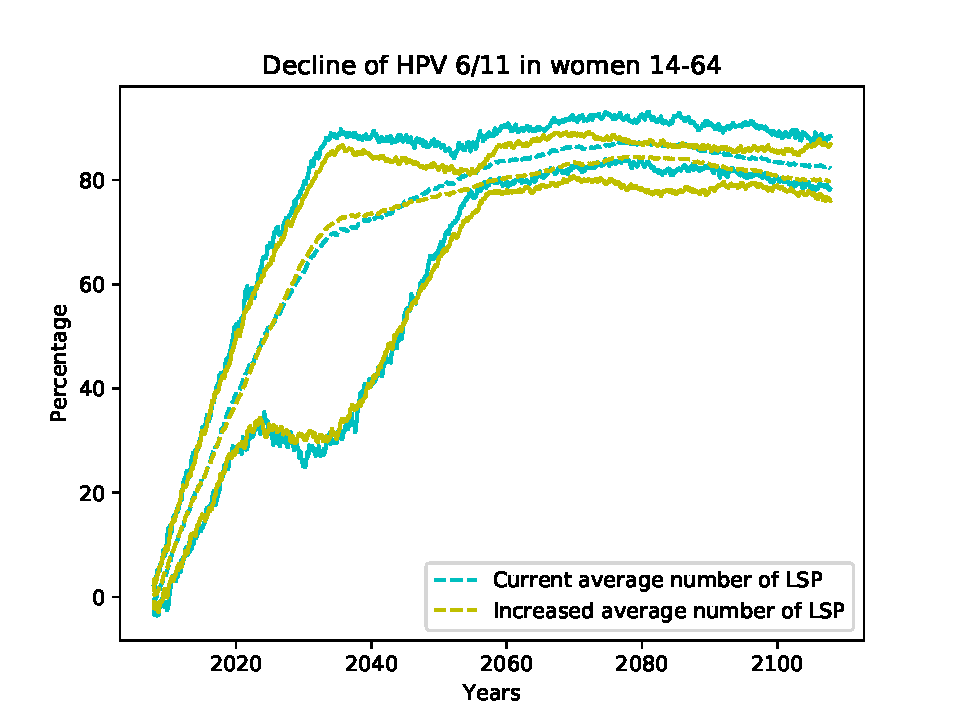
\includegraphics[width=0.5\linewidth]{IMGs/12.-Aumento_LSP/verr_muj.pdf}  \\ 
		Decline oncogenic HPV women	& Decline HPV 6/11 women \\ 
	\end{tabular} 
	\caption{Comparative of the decline of HPV in case the global average number of LSP increases in $4$. In the current vaccination scenario (vaccinating only girls with a coverage of $70\%$, there are not significant changes in declines.}
	\label{fig:compara_k}
\end{figure}

As we can see, the increase in 4 the global number of average LSP does not provide any substantial change in the decline of the HPV infections.

The simulation performed assumes a noticeable increase in the number of average LSP. However, it does not have a significant effect on the decline of the HPV infections. In the Figure 2 of paper \cite{acedo2011using} the authors study the average number of contacts for the transmision dynamics of the Respiratory Sincitial Virus (RSV) and takes valus greater than 25 in which the epidemic does not fade away. Therefore, in order to have significant changes in the decline of HPV infection, it would be necessary to increase the number of average LSP to values close to the average number of LSP of MSM, 39 \cite{Durex2002}. Nevertheless, for these numbers of LSPs the STDs would become as the influenza or RSV and the herd immunity effect would dissapear.

The present simulation can be interpreted as a sensitivity analysis that supports the robustness of this study.
